The given curve can be expressed as 
\begin{align}
    &x^2+2y-3=0\\
    \implies \vec{V} = &\myvec{1&0\\0&0},\; \vec{u} = \myvec{0\\1},\; \vec{f} = -3
\end{align}

Since $\abs{\vec{V}} = 0$, the given curve represents a parabola. The eigenvalues are given by 
\begin{equation}
    \lambda_1 = 0, \; \lambda_2 = 1
\end{equation}

with corresponding eigenvectors 
\begin{align}
    \myvec{1&0\\0&0}\vec{x} = 0 \implies \vec{p}_1 = \myvec{0\\1}\\
    \myvec{0&0\\0&-1}\vec{x} = 0 \implies \vec{p}_2 = \myvec{1\\0}
\end{align}

To find the vertex of the parabola,
\begin{equation}
    \myvec{\vec{u}^\top+\kappa \vec{p}_1^\top\\\vec{V}}\vec{c} = \myvec{-\vec{f}\\\kappa \vec{p}_1-\vec{u}}
\end{equation}

where, $\kappa = \vec{u}^\top\vec{p}_1 = 1$
\begin{align}
    \implies \myvec{0&2\\1&0\\0&0}\vec{c} &= \myvec{3\\0\\0}\\
    \implies \vec{c} &= \myvec{0\\1.5}
\end{align}

Now to evaluate the direction vector $\vec{m}$,
\begin{align}
    \vec{m}^\top (\vec{V}\vec{q}+\vec{u}) &= 0\\
    \implies \vec{m}^\top \myvec{\myvec{1&0\\0&0}\myvec{1\\1}+\myvec{0\\1}} &= 0\\
    \implies \vec{m}^\top \myvec{1\\1} &= 0\\
    \implies \vec{m} &= \myvec{-1\\1}
\end{align}

The normal is obtained as 
\begin{align}
    \vec{m}^\top (\vec{x}-\vec{q}) &= 0\\
    \implies \myvec{-1&1}\myvec{\vec{x}-\myvec{1\\1}} &= 0\\
    \implies \myvec{-1&1}\vec{x} &= 0
\end{align}

The above results are verified in Fig. \ref{sep/2/68/plot}. 
\begin{figure}
    \centering
    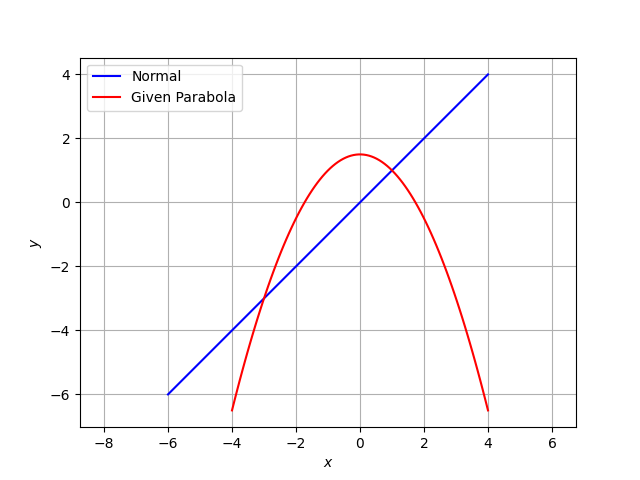
\includegraphics[width=\columnwidth]{solutions/sep/2/68/figures/figure.png}
    \caption{Plot of the normal}
    \label{sep/2/68/plot}
\end{figure}

